\documentclass{letter}

\usepackage[left=0.75in, right=0.75in, top=1.1in, bottom=0.75in]{geometry}
\usepackage{fancyhdr, amsmath, amssymb, mathtools, xcolor, graphicx, listings, mathpazo}
\graphicspath{{.}}

\pagestyle{fancy}
\fancyhf{}
\rhead{Page \thepage}
\chead{AMSC808N Homework 6}
\lhead{Tyler Hoffman}
\setlength{\headsep}{0.2in}

\newcounter{problem}
\newcounter{subproblem}[problem]
\newcounter{solution}

\renewcommand{\thesubproblem}{(\alph{subproblem})}

\newcommand{\Problem}[2]{%
	\stepcounter{problem}%
	\leftskip=0pt%
	\theproblem.~\textbf{{#1.}} #2 \par%
}

\newcommand{\Subproblem}[1]{%
	\stepcounter{subproblem}%
	\leftskip=15pt%
	\thesubproblem~ #1 \par%
}

\newcommand{\Solution}[1]{%
	\textbf{Solution.} #1 \par%
}

\newcommand{\Due}[1]{\textbf{Due: #1} \par}

\newcommand{\UNFINISHED}{\textbf{\color{red} UNFINISHED}}
\newcommand{\CHECK}{\textbf{\color{orange} CHECK ME}}

\newcommand{\iu}{{i\mkern1mu}}
\newcommand{\T}{\intercal}
\newcommand{\R}{\mathbb{R}}

\DeclareMathOperator{\diag}{diag}
\DeclareMathOperator{\rank}{rank}
\DeclareMathOperator{\nul}{nul}
\DeclareMathOperator{\tr}{tr}

\usepackage{hyperref}
\begin{document}
    \Due{3 Dec 2020}

    \Problem{Depth-first search}{Implement the DFS to check experimentally the theoretical result for the Poisson random graph with mean degree $z = p(n-1)$. \begin{itemize}
        \item The fraction $S$ of vertices in the giant component is the largest solution of $S = 1 - \exp(-zS)$.
        \item Let $v$ be a randomly chosen vertex from a non-giant component. The average size of the component to which $v$ belongs is \begin{align*}
            \langle s \rangle = \frac{1}{1- z + zS}.
    \end{align*}
    \end{itemize} Proceed as follows. Program the DFS from scratch. Set the number of vertices $n = 1000$. Define a grid of values of $z$ ranging between 0 and 4. For each $z$, generate $r = 100$ random graphs $G(n,p)$ where $p = z/(n-1)$. For each graph, use the DFS to find its connected components. Calculate $\langle s(z) \rangle$ and $S(z)$. Make two figures: \begin{itemize}
        \item Figure 1: find numerically and plot the theoretical values $S(z)$ versus $z$. Also plot experimentally found values for $S(z)$.
        \item Figure 2: plot the theoretical value for $\langle s(z) \rangle = [1 - z + zS(z)]^{-1}$ and the experimentally found values for $\langle s(z) \rangle$.
    \end{itemize} Comment on your findings. Link files with your codes.}
    \Solution{All my codes can be found at \href{https://github.com/thoffman1/amsc808n/tree/master/hws/hw6}{this Github link}. The file \texttt{graphs.py} has the \texttt{Node} and \texttt{Graph} classes that I used to run the algorithms. When the \texttt{Graph} class is initialized, it creates all the required \texttt{Node}s, stores them in a list (set), and randomly connects the nodes by creating a random adjacency matrix. I used an adjacency matrix as \texttt{numpy} is faster than built-in Python data structures; creating the linked lists needed for the adjacency list implementation would have been more efficient in C but did not make sense in Python. The \texttt{Graph} class has a \texttt{DFS()} instance method which returns the roots of the depth-first forest and also updates an instance variable with the list of roots for easy access later. In a separate notebook (\texttt{analysis.ipynb}), I ran the computations needed for this problem and plotted the figures. To calculate the theoretical $S(z)$, I used the \texttt{broyden1} nonlinear solver from the \texttt{scipy.optimize} module.

    The theoretical curves and empirical curves line up quite nicely in these figures. In Figure 1 we see especially nice agreement between the theoretical and empirical results. The phase shift appears at $z = 1$ as predicted by the theory and the curves effectively lay on top of each other for the rest of the plot. In the $\langle s(z) \rangle$ plot, we see similar agreement away from $z = 1$ and good agreement near the peak at $z = 1$, although the two diverge slightly in this vicinity. This is likely due to the extreme randomness being experienced at this average degree---when $z$ is near 1, the component sizes will fluctuate dramatically, so that even averaging may not perfectly reflect them.

    \begin{center} 
        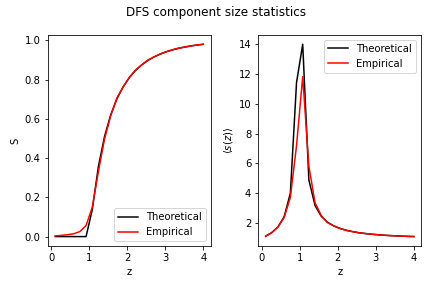
\includegraphics{../code/dfsstats.png} \\
        Figure 1 (left): Theoretical versus empirical values for $S(z)$, $z \in (0, 4]$. \\
        Figure 2 (right): Theoretical versus empirical values for $\langle s(z) \rangle$, $z \in (0, 4]$.
    \end{center}}

    \Problem{Breadth-first search}{Implement the BFS to obtain estimates for the average length of shortest paths in the Poisson random graph \begin{align*}
        \ell \simeq \frac{\log(n)}{\log(z)}.
    \end{align*} Proceed as follows. Program the BFS from scratch. Set $z = 4$ so that almost all vertices belong to the giant component. For $n = 2^p$, $p = 10, 11, 12, 13$, generate a random graph $G(n,p)$. Randomly select $r = 100$ vertices and use each of them as a seed for the BFS. Average the found path lengths and find $\ell(n)$. Plot the found $\ell(n)$ versus $n$ as well as the theoretical estimate above. Comment on your observations. Link files with your codes.}
    \Solution{Again, I programmed the algorithm in Python and used an adjacency matrix. The \texttt{Graph} class has a \texttt{BFS(s)} instance method which accepts as an argument \texttt{s}, a source vertex. My driver code is in \texttt{analysis.ipynb}, where I do the setup as suggested: for each $n$, create one random graph and use $r = 100$ randomly chosen source vertices to run \texttt{BFS} on. The \texttt{BFS} method, as written, records all the path lengths it finds in the dictionary \texttt{path\_lengths} and returns the average path length in the dictionary. If the source vertex has no adjacent nodes, the method returns 0. The driver code averages the average path lengths over the trials and produces the array \texttt{empL} (empirical $\ell$), which I then plotted against the theoretical $\ell(n)$ (Figure 3).

    We see nice agreement between the theoretical and empirical values in Figure 3 on semilog axes. As $n$ grows, the two curves diverge slightly, but as mentioned on Piazza the match is not very good for these choices of $n$.
    
    \begin{center}
        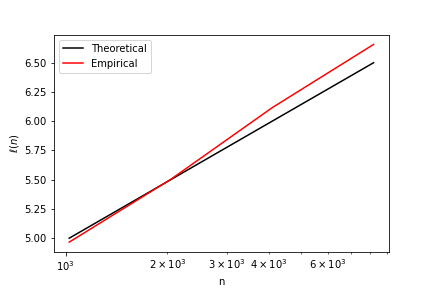
\includegraphics{../code/bfsstats.png} \\
        Figure 3: Theoretical versus empirical average path lengths ($\ell(n)$) for $n = 2^p$, $p = 10, 11, 12, 13$ plotted on semilog axes in $n$ (since we scaled $n$ logarithmically to begin with).
    \end{center}}

    \Problem{Reading}{Read sections II.A,C,D of the given paper by Newman, Strogatz, and Watts. Consider a random graph with a prescribed degree distribution $p_k$. Let $v$ be a randomly chosen vertex from a non-giant component. Write a book report with a detailed derivation of the formula for the average size of the component to which $v$ belongs, excluding the giant component: \begin{align*}
        \langle s \rangle = 1 + \frac{zu^2}{[1-S][1-G'_1(u)]}.
    \end{align*}}
    \Solution{In II.A of the paper, the authors begin by defining $G_0(x) = \sum_{k=0}^\infty p_kx^k$ to be the generating function of the degree distribution $p_k$. Since $G_0$ is a generating function, we necessarily have $G_0(1) = 1$. To ensure that the appropriate assumptions are satisfied, the authors restrict their analysis to the region $|x| \leq 1$ and elaborate on a few properties of generating functions: \begin{itemize}
        \item \emph{Derivatives.} For a generating function $G$ we have that \begin{align*}
            p_k = \frac{1}{k!}\left.\frac{d^kG}{dx^k}\right|_{x=0}
        \end{align*} i.e. each probability is generated by a derivative of $G$.
        \item \emph{Moments.} The $n$th moment of the distribution $p_k$ can be computed using the generating function $G$ as follows: \begin{align*}
            \langle k^n \rangle = \sum_k k^np_k = \left[\left(x\frac{d}{dx}\right)^nG(x)\right]_{x=1}.
        \end{align*}
        \item \emph{Powers.} The power of a generating function is the sum \begin{align*}
            (G(x))^n = \sum_k \sum_{i + j = k} p_ip_jx^k.
        \end{align*}
    \end{itemize} For conciseness, denote $z = \langle k \rangle = G'_0(1)$ to be the mean degree of a vertex.
    
    One other distribution that is of relevance to us is the distribution of (excess) outgoing edges from a random vertex, given that we just reached it from a random edge. This is given by \begin{align*}
        G_1(x) := \frac{G'_0(x)}{G'_0(1)} = \frac{1}{z}G'_0(x)
    \end{align*} as we remove one power of $x$ from $G_0$ to account for the edge we used to get to it and then normalize. These are the tools we'll need to derive the given formula for the average size of the component to which a random vertex belongs.
    
    Proceeding from this point, we define $H_1(x)$ to be the generating function for the distribution of the sizes of the non-giant components obtained by choosing a random vertex. Denote by $q_k$ the probability that an initial vertex has $k$ edges originating from it. Then, assuming that all the non-giant components contain no cycles (i.e. are tree-like), we will have the following self-consistency equation for $H_1(x)$: \begin{align*}
        H_1(x) = xq_0 + xq_1H_1(x) + xq_2(H_1(x))^2 + \dots 
    \end{align*} which is obtained by summing each ``tree'' probability recursively. Notice now that $q_k$ is the same coefficients we needed when defining $G_1$ earlier. As a result, we have \begin{align*}
        H_1(x) = xG_1(H_1(x))
    \end{align*} and also when including the giant component we obtain \begin{align*}
        H_0(x) := xG_0(H_1(x)).
    \end{align*} These equations, while theoretically tractable, are in practice extremely difficult to solve. The authors suggest a few methods for using symbolic computer programs or contouur integration to obtain the results.
    
    The challenge, then, is to find a closed-form expression for the average sizes of components that vertices belong to. In the case with no giant component, this is simply $H'_0(1)$ as this is the first moment of the desired distribution. Here, the authors derive a formula for $\langle s \rangle$ in terms of the average number of first and second neighbors of a vertex (in class, we obtained a quantity in terms only of the average vertex degree). However, things quickly get messier when there is a giant component. 
    
    When there is a giant component, $H_0(1)$ is no longer equal to 1 as it generates the distribution of component sizes for all the non-giant components. Hence, $H_0(1) = 1 - S$ where $S$ is the fraction of the graph occupied by the giant component. As a result, we can use the pair of equations derived earlier to get that $S = 1 - G_0(u)$ where $u$ is the smallest real solution of $u = G_1(u)$ (that is, $u = H_1(1)$): \begin{align*}
        H_0(1) = 1 - S = G_0(H_1(1)) \implies 1 - G_0(H_1(1)) = S \implies S = 1 - G_0(u).
    \end{align*}
    
    Therefore, $\langle s \rangle$ is the average size of the non-giant component and is equal to $H'_0(1)$ normalized by $H_0(1)$ as $H_0(1) \neq 1$. Using the product rule, this looks like \begin{align*}
        \langle s \rangle &= \frac{H'_0(1)}{H_0(1)} = \frac{1}{H_0(1)}\left[G_0(H_1(1)) + \frac{G'_0(H_1(1))G_1(H_1(1))}{1 - G'_1(H_1(1))}\right] \\
        &= \frac{1}{1 - S}\left[G_0(u) + \frac{G'_0(u)G_1(u)}{1 - G'_1(u)}\right] \\
        &= \frac{1}{1 - S}\left[1 - S + \frac{G'_0(u)u}{1 - G'_1(u)}\right] \\
        &= 1 + \frac{zu^2}{[1 - S][1 - G'_1(u)]},
    \end{align*} as desired since $G_0(u) = 1 - S$ and $G'_0(u) = zu$.}
\end{document}